%!TEX root = ../../thesis.tex

\section{Keplerian Orbits}
\label{sec:keplerian_orbits}
When two bodies are in orbit (two stars or a star and a planet) they orbit about their common centre of mass.
Their 3-dimensional motion can be derived with a combination of Newton's universal law of gravitation, and represented through Kepler's laws.
The full derivation is quite long and can be commonly found in several celestial mechanics texts~\citep[e.g.][]{moulton_introduction_1914, perryman_exoplanet_2011, fitzpatrick_introduction_2012}.
The notes given here mainly follow~\citet{bozza_methods_2016}.

\begin{figure}
    \centering
    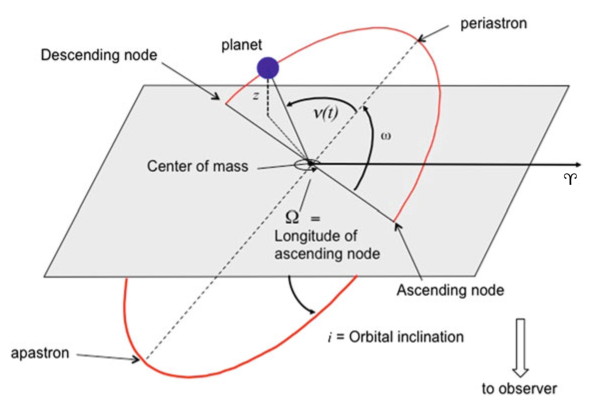
\includegraphics[width=0.6\linewidth]{figures/fundamental_rv/orbit_diagram2.pdf}
    \caption[The basic elements of the Keplerian orbit.]{The basic elements of the Keplerian orbit.
        Adapted from~\citet{bozza_methods_2016}.}
    \label{fig:orbitdiagram}
\end{figure}

\Cref{fig:orbitdiagram} shows the basic elements of the Keplerian orbit.
There are several parameters required to situate the orbit in space.
When dealing with exoplanetary systems, there is a \textit{reference plane}, usually considered as tangential to the celestial sphere, that cuts the orbital plane with a \textit{line of nodes}.
The \textit{ascending node} is the point on the plane at which the body crosses the reference plane moving away from the observer, and is defined relative to the vernal reference point, \Aries, with the \textit{longitude of the ascending node}, $\Omega$, setting the orientation.

To fully parametrize a Keplerian orbit requires seven parameters.
These are: \(a\) the semi-major axis of the elliptical orbit, \(e\) the orbital eccentricity, \(P\) orbital period, $T_0$ the \emph{time of periastron passage}, \(i\) orbital inclination relative to the line of sight, \(\omega\) the \emph{argument of periastron}, and $\Omega$.
From {RV} measurements alone all of these parameters except for \(i\) and $\Omega$ can be determined.
$\Omega$ is irrelevant for determining the orbital mass, but the inclination \(i\) is very important as it affects the projection of the velocity towards the observer, and as such affects the mass one ultimately aims to measure.

With a two body system with masses \Mone{} and \Mtwo{}, under the force of gravity, their orbits are elliptical orbits about their barycentre mass, as seen in \cref{fig:eclipesorbit}.
In polar coordinates the ellipse of an orbit about the centre of mass (located at the focus $\textrm{F}_1$) is described by:
\begin{equation}
    r = \frac{a(\oneminusetwo)}{1 + e \cos{\nu(t)}},
\end{equation}
where \(a\) is the length of the semi-major axis for the body, \(e\) is the eccentricity, $\nu$ is the \emph{true anomaly} the angle between the current position of the orbiting body and periastron, as seen from the main focus of the orbital ellipse.

The true anomaly is not only a function time, \(t\), but also the orbital period \(P\), the \emph{time of periastron passage}, \(T_0\), and eccentricity.
It is geometrically related to the eccentric anomaly:
\begin{equation}
    \cos{\nu(t)} = \frac{\cos{E(t)}}{1 - e \cos{E(t)}}
\end{equation}
which can be numerically determined from the mean anomaly \(M(t)\):
\begin{equation}
    M(t) = \frac{2 \pi}{P}(t - T_0) = E(t) - e \sin{E(t)}
\end{equation}
The mean anomaly is the angle for the average orbital motion of the body at a time after periastron passage \(t-T_0\).

\begin{figure}
    \centering
    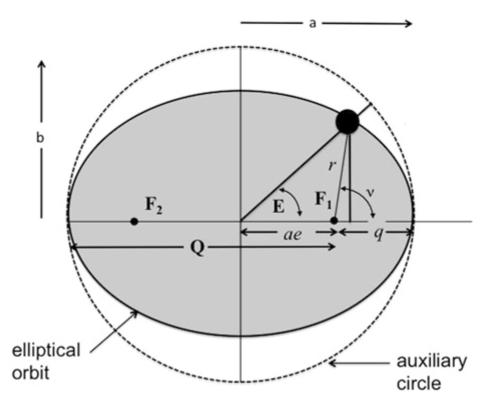
\includegraphics[width=0.55\linewidth]{figures/fundamental_rv/eclipes_orbit2.pdf}
    \caption[Elements of an elliptical orbit.]{Elements of an elliptical orbit about the common centre of mass \(\textrm{F}_1\).
        {\(\nu\)} is the angle to the position of the orbiting body from the periapse (closest point to barycentre).
        The auxiliary circle has a radius equal to the semi-major axis of the ellipse.
        Adapted from~\citet{bozza_methods_2016}.}
    \label{fig:eclipesorbit}
\end{figure}

From Kepler's second law\footnote{Orbit sweeps out equal areas in equal times} \(\frac{1}{2} r^{2} d\nu/dt\) = constant, while in one full period P, the total area of the ellipse \(\pi a^{2}{(\oneminusetwo)}^{1/2} \) will be covered, leading to:
\begin{equation}
    r^{2} \frac{d\nu}{dt} = \frac{2\pi a^{2}(\oneminusetwo)^{1/2}}{P} \label{eqn:kepler_area}
\end{equation}

The radial velocity is the change in \(r\) along the line of sight \(z\).
The component of \(r\) along the line of sight (from \cref{fig:orbitdiagram}) is:
\begin{equation}
    r_z =  r_1 \sin{(\nu_1(t) + \omega)}\sin{i} + \gamma \label{eqn:r_z}
\end{equation}
where \(\gamma\) is the mean velocity of the barycentre, and the subscripts `1' refers to the star.
Differentiating \cref{eqn:r_z} and substituting in \cref{eqn:kepler_area} leaves the common {RV} equation:
\begin{align}
    {RV} = \dot{r}_z &= \frac{2 \pi a_1 \sin{i}}{P{(\oneminusetwo)}^{1/2}} [\cos{(\nu(t) + \omega)} + e\cos{\omega}] + \gamma  \label{eqn:rv_equation} \\
     &= \kone [\cos{(\nu(t) + \omega)} + e\cos{\omega}] + \gamma,
\end{align}
where several parameters and constants have been condensed into $\textrm{K}$, referred to as the \emph{semi amplitude}.
In this case \Kone{} is the semi amplitude for the star.
From the above equation it can be seen that a fit to the {RV} time series allow for the parameters \Kone{}, \(P\), \(T_0\), \(\omega\), \(e\), and \(\gamma\) to be derived.

\subsection{Mass function}
Once the orbital parameters have been determined then it is possible to determine the mass function of the system.
From the centre of mass the distance between the two bodies is \(a = a_1 + a_2\) where $a_1$ and $a_2$ are the respective distances to the barycentre with the subscripts `1' and `2' refer to the star and planet (or companion star), respectively.
The value \(\mone a_1 = \mtwo a_2\) can allow these re-arrangements:
\begin{equation}
    a = a_{1} (1 + \frac{a_{2}}{a_{1}}) = a_{1}(1 + \frac{\mone}{\mtwo}) = \frac{a_{1}}{\mtwo} (\mone + \mtwo)
\end{equation}

Kepler's third law (\({G (\mone + \mtwo)}/{4\pi^{2}}= {a}^{3}/{P}^{2}\)) can be written as:
\begin{equation}
    \frac{G (\mone{} + \mtwo{})}{4\pi^{2}} = \frac{a_{1}^{3}}{P^{2}}{\left(\frac{\mone{} + \mtwo}{\mtwo}\right)}^{3}
\end{equation}
replacing $a_{1}$ with $\kone$ from \cref{eqn:rv_equation} results in the \emph{mass function}, $f(M)$:
\begin{equation}
    f(M) = \frac{{(\mtwosini)}^{3}}{{(\mone{} + \mtwo{})}^{2}} = \frac{\kone{}^{3} P {(\oneminusetwo)}^{3/2}}{2 \pi G} \label{eqn:mass_function}
\end{equation}
This function can be determined directly from the measurable parameters \(P\), \(e\) and \Kone{}.
It shows that to determine the planet mass,\Mtwo{}, knowledge of the stellar mass, \Mone{}, must also be known.
It can be seen from \cref{eqn:mass_function} that the true mass of the planet \Mtwo{} is not obtained but only the projected mass \Mtwosini{}.

For a planetary companion the approximation \(\mtwo{} \ll \mone{}\) can be made and for circular orbits (\(e=0\)) the radial velocity semi-amplitude can be re-written as:
\begin{equation}
    \kone{}=\frac{28.4}{\sqrt{\oneminusetwo}} \frac{\mtwosini}{\mjup} {\left(\frac{\mone}{\modot}\right)}^{-2/3} {\left(\frac{P}{1 \si{yr}}\right)}^{-1/3}  [\mps] \label{eqn:k_relation}
\end{equation}

This can be used to calculate the {RV} amplitude created by different mass planets in various circular orbits as given in \cref{tab:rv_amplitudes}.
The recently commissioned ESPRESSO optical spectrograph is designed with the goal of achieving 10\cmps{}, which is the level of precision required to detect an Earth mass planet in a one year orbit round a Sun-like star.

%!TEX root = ../thesis.tex

\begin{table}
    \centering
    \caption{The RV semi-amplitude induced by the plants with different masses and periods around a 1~\Msun-mass star.}
    \begin{tabular}{lcccc}
        \toprule
        \Mtwo{}                        & \Kone{}($P = 3$\,d) & \Kone{}($P = 1$\si{yr}) & \Kone{}($P = 5$\si{yr}) & \\
        \midrule
        \Mjup                             & 140.8 & 28.4 & 16.6  & \mps{}\\
        \(\textrm{M}_{Nep}\)  & 7.60   & 1.53 & 0.90  & \mps{}\\
        \Modot                           & 44.3   & 8.9   & 5.2  & \cmps{}\\
        \bottomrule
    \end{tabular} \label{tab:rv_amplitudes}
\end{table}


If there is more than one companion/planet then there will be a gravitational influence between each other and their orbits become non-Keplerian, i.e.\ an N-body problem~\citep[e.g.][]{chenciner_three_2007, correia_chaotic_2018, gao_numerical_2018, lillo-box_troy_2018, leleu_coorbital_2019}.
Assuming that the gravitational influence between companions is negligible, the {RV} signal observed in the host star can be treated as just a sum of tugs from each companion.
For the two instances in this work where the target star has two companions, the companions will be treated separately, as if they were alone.


\subsection{Binary mass ratio}
\label{subsec:binary_mass_ratio}
In the above equation {RV} of the companion has not yet been addressed.
\cref{eqn:rv_equation} above is the {RV} of the star in an elliptical orbit around the centre of mass between it and its companion.
Similarly the elliptical orbit of the planet around the centre of mass is given by:
\begin{equation}
    {RV_{2}} = \ktwo{} [\cos{(\nu(t) + \omega_{2})} + e\cos{(\omega_{2})}] + \gamma, \label{eqn:rv2_equation}
\end{equation}
where \(\omega_{2} = \omega + 180^\circ\) due to the phase difference between the two components, resulting in the relative velocity (ignoring \(\gamma\)) of the companion being opposite the star and:
\begin{equation}
    \ktwo  = {\left(  \frac{2 \pi G}{P{(\oneminusetwo)}^{3/2}} \right)}^{1/3} \frac{\mone \sin{i}}{{(\mone + \mtwo)}^{2/3}} = \frac{2 \pi a_2 \sin{i}}{P{(\oneminusetwo)}^{1/2}} \label{eqn:ktwo}
\end{equation}

The orbits of the host and companion are directly related through the mass ratio of the star and companion:
\begin{equation}
q = \frac{\mtwo}{\mone} = \frac{\kone}{\ktwo} = \frac{RV_{1}}{RV_{2}}  \label{eqn:q_ratio_K2}. %= \frac{r_2}{r_1}??
\end{equation}

Typically in exoplanet detections the companion (planet) is too faint to measure the planetary velocity.
In fact exoplanet field originates from, and is the lower limit of, the study of binary stars, revolutionized by works such as~\citet{duquennoy_multiplicity_1991}.
In double lined spectroscopic binary the spectrum of both stars can be identified in the blended spectra and the {RV} of both star and companion can be measured and monitored over the orbit.
With both velocities the mass ratio of the binary can be found.
The individual masses however are still not determinable due to the inclination $\sin{i}$ of the orbit.

In \cref{cha:direct_recovery} the detection of the faint spectra of known companions is attempted, in order to determine the velocity change of the companion and hence the mass ratio.
To help with the analysis and simulations the known orbital parameters (see \cref{tab:orbitparams,tab:star_params}) are used along with the companion mass (\Mtwo{} or \Mtwosini{}) to predict or estimate the {RV} of the companion using \cref{eqn:q_ratio_K2,eqn:rv2_equation}.
Note, that for the targets in which only the minimum mass (\Mtwosini{}) is known and used in the mass ratio, this will result in the maximum {RV} semi amplitude for the companion.
The estimated \Ktwo{} for each companion is provided in \cref{tab:estimated_rv} while the {RV} for both components at the time of each observation is provided in \cref{tab:observations}.
